\documentclass[11pt]{article}
%%%%%%%%%%%%%%%%%%%%%%%%%%%%%%%%%%%%%%%%
\usepackage{amsmath}
\usepackage{verbatim}
\usepackage[usenames,dvipsnames]{color}
\usepackage{setspace}
\usepackage{lscape}
\usepackage{longtable}
\usepackage[top=1.25in,bottom=1.25in,left=1in,right=1in]{geometry}
\usepackage{graphicx}
\usepackage{epstopdf}
\usepackage{epsfig}
\usepackage{fancyhdr}
\usepackage{booktabs}
\usepackage{dcolumn}
\usepackage{arydshln}
\usepackage{natbib}
\usepackage{tabularx}
\usepackage{subfigure}

{\newcommand{\districts}{  28,475}
{\newcommand{\provinces}{   2,282}
{\newcommand{\countries}{     151}
 % commands for counts of observations

\newtheorem{proposition}{Proposition}
\newtheorem{corollary}{Corollary}

\setcounter{MaxMatrixCols}{10}
\newcolumntype{d}[1]{D{.}{.}{-2.#1}}
\newenvironment{proof}[1][Proof]{\noindent\textbf{#1.} }{\ \rule{0.5em}{0.5em}}
\setlength{\columnsep}{.2in}
%\psset{unit=1cm}

\def\sym#1{\ifmmode^{#1}\else\(^{#1}\)\fi}

\begin{document}
\begin{titlepage}
\vspace{2in} \noindent {\large \today}

\vspace{.5in} \noindent {\Large \textbf{\strut The role of land in temperate and tropical agriculture}}

\vspace{.25in} \noindent {\large T. Ryan Johnson}

\vspace{.05in} \noindent Washington University

\vspace{.25in} \noindent {\large Dietrich Vollrath}

\vspace{.05in} \noindent University of Houston

\vfill \noindent \textsc{Abstract} \hrulefill

\vspace{.05in} \noindent We document that the importance of land differs significantly in temperate and tropical agriculture. Using district level data (i.e. 2nd-level administrative units), we estimate the elasticity of agricultural output with respect to land by examining variation in rural density and inherent agricultural productivity. The elasticity in areas with temperate agriculture (0.23) is significantly higher than in areas with tropical agriculture (0.13). A two-sector model shows that the high elasticity in temperate areas makes their living standards more sensitive to shocks in population growth and technology. We confirm these predictions using evidence from the post-war mortality transition.
 
\vspace{.1in} \hrule

\vspace{.5in} \noindent {\small JEL Codes: O1, O13, O44, Q10}

\vspace{.1in} \noindent {\small Keywords: land constraints, land elasticity, agricultural productivity, agro-climatic, temperate, tropical}

\vspace{.1in} \noindent {\small Contact information: 201C McElhinney Hall, U. of Houston, Houston, TX 77204, devollrath@uh.edu. We thank Francesco Caselli, Martin Fiszbein, Oded Galor, Remi Jedwab, Nippe Lagerl{\"o}f, Debin Ma, Stelios Michalopolous, Nathan Nunn, {\"O}mer {\"O}zak, Stephen Smith, Enrico Spolaore, Joachim Voth, and David Weil, as well as seminar participants at the London School of Economics, Texas A\&M Ag. Econ, the Brown Conference on Deep-rooted Determinants of Development, George Washington University, and the University of Houston brown bag series for their comments. This paper previously circulated under the title ``How Tight are Malthusian Constraints?''. All errors remain our own.}
\end{titlepage}

\pagebreak 

\section{Introduction}
\onehalfspacing 
Agricultural production relies on the use of a finite (or inelastically supplied) resource, land. But that reliance on land, relative to the reliance on non-land inputs like labor or capital, need not be identical in different locations. To be specific, the elasticity of agricultural output with respect to land may differ by climate or the type of crops suitable for production. This land elasticity is relevant to any study of growth and development that includes an agricultural sector, as with the mild assumption of constant returns to scale, one minus the land elasticity tells us how sensitive agricultural output is to the use of the non-land inputs. This in turn determines how much capital and labor will move out of, or into, agriculture in response to shocks to productivity or population. Differences in the land elasticity by crop or climate thus imply differences in the reaction of economies to those shocks, with implications for studies of comparative development, structural change, Malthusian stagnation and the take-off to sustained growth, and long-run growth prospects with finite resources.\footnote{Agriculture and land feature in stories of divergence across global regions \citep{kp2001,galor2008trading,vollrath2011,vv08,vv13,cs2015}. On structural change, see \cite{Gollin:2007oq,Restuccia:2008hc,weilwilde2009,Gollin:2010ys,ev2016clim}. For Malthusian stagnation, see \cite{ashraf2010dynamics} for a baseline model, and \citet{Galor:2011uq} for a review of major contributions to the literature on the take-off to growth \citep{gw00,galor2002natural,Hansen:2002fk,doepke2004accounting,cs2005,lagerlof2006,craftsmills2009,strulik2008population}. On the relevance of resources for long-run growth, see \cite{perettovalente2015}.} 

In this paper, we estimate the agricultural land elasticity, and show that it varies across different agricultural regions and climate types. Estimating the parameter(s) of a production function is not straightforward, for the standard reasons that total factor productivity is unobserved and inputs may be mis-measured. To address this, we first develop a method for estimating the aggregate land elasticity using the relationship between the density of agricultural workers and the potential agro-climatic yield across small geographic units (e.g. 2nd-level districts within provinces/states). Our method allows for inputs other than land and labor in the production function, but does not require us to identify exactly what those other inputs are, avoiding mis-measurement issues. We use agro-climatic yield data to give us a source of exogenous variation in productivity, and combine that with measures of district-level development (e.g. night lights and urbanization) to control for other unobservable elements of agricultural productivity. In addition, our estimates are made using only within-province variation across districts, meaning that unobservable variation in productivity \textit{across} provinces, as well as \textit{across} countries, is removed from the estimates.\footnote{There are two main studies that focus on the spatial distribution of labor (in general) and economic activity. The first is \citet{mfm2014}. Those authors examine the growth of urbanization at the grid-cell level over the last two-thousand years. The second is \citet{hssw2016}, who examine the spatial distribution of economic activity (associated with urbanization) at the grid-cell level using night lights, relating it to geographic characteristics associated with either agriculture or trade.} 

We assemble data at the district level for rural population density in the year 2000 from the HYDE database \citep{hyde31}, and combine that with a measure of potential agro-climatic yield in districts built from the data of \citet{galorozak2016}. As in their work, our measure is built on constraints plausibly unaffected by human activity (e.g. soil quality and length of growing season) from the Global Agro-Ecological Zone (GAEZ) project \citep{gaez}, combined with information on the calorie content of various crops. Grid cell potential caloric yields are aggregated to the district level to serve as our measure of agro-climatic yield.

In the end, we have a dataset of\districts \ districts, coming from\provinces \ provinces in\countries \ countries. Using this data, we divide districts into regions defined by the types of crops they are capable of growing, and estimate a separate land elasticity for each region. The ``temperate'' region (i.e. it includes districts that can grow crops such as wheat, barley, and rye) is distinguished from a ``tropical'' region (i.e. it includes districts that can grow crops such as rice, cassava, and pearl millet). Our classification allows us to distinguish temperate and tropical districts within countries, so that we do not have to assume that agriculture within a heterogenous country (e.g. the U.S., China, Brazil) has a homogenous land elasticity.  

Our baseline estimate is that the land elasticity is 0.225 in temperate districts. In contrast, our baseline estimate of the land elasticity is only 0.130 for tropical districts. Our initial definition of temperate and tropical are based on suitability for growing specific crops, and not on direct temperature or precipitation regimes. Nevertheless, the approximate 0.10 difference in the land elasticity holds up across alternate definitions of what constitutes temperate and tropical regions. 

Our results are robust to the exclusion of districts that contain large urban areas, the exclusion of districts from any developed country, or the exclusion of districts that appear to depend more on pastoralism than crop production. Further, the results are consistent if we use alternative measures of rural population density, alternative measures of the potential agro-climatic yield, or alternative measures of the area of agricultural land used within a district. In all cases, the aggregate land elasticity in temperate districts remains approximately 0.10 higher than in tropical districts, and the difference remains statistically significant.\footnote{These results are consistent with the work of \citet{Ruthenberg:1976zr} and \citet{bray1994}, who discuss the inherent differences in the response of tropical crops (rice, in particular) to the application of labor. They both cite the relatively \textit{high} elasticity of output with respect to labor in tropical agriculture, which is consistent with a low elasticity of output with respect to land.} 

Relative to the existing literature, our approach to estimating the aggregate land elasticity has several advantages. The standard approach has been to use country-level panel data \citep{Hayami:1970ly,Hayami:1985cr,cpr1997,mm2001,Mundlak:2000dq,mbl2012,et2013mango} to estimate agricultural production functions, with a common set of coefficients across countries for each input, including land. Issues arise with unobserved productivity, the measurement of non-land inputs, and the assumption that coefficients are common to all countries. Some have examined heterogeneity in these coefficients \citep{gg2003,Wiebe2003Resource-Qualit} by continent, while others have attempted to estimate country-level coefficients using factor analysis to address unobserved productivity \citep{et2013mango,ev2016clim}. Compared to this, our district-level data allows us to control for unobserved country and province-level effects, and the use of agro-climatic yield data gives us a better measure of productivity. 

As may be clear, we are not estimating the elasticity of a \textit{farm}-level production function, but rather for an \textit{aggregate} production function. Farm-level estimates of the land elasticity would not necessarily be informative about the aggregate production function, given that those estimates would refer to farmers using a given technique, while the aggregate function can be thought of as an envelope across techniques available to farmers \citep{Hayami:1970ly}.\footnote{More general treatments of this idea can be found in \citet{houthakker1955} and \citet{jones2005}. In short, the farm-level land elasticities may not be informative on the aggregate land elasticity, and farm-level production functions may well take on different forms (i.e. Leontief verus Cobb-Dougals) than the aggregate function.} The aggregate land elasticity is a useful parameter for studying the role of the agricultural sector and its interaction with other sectors during development, as we discuss below, while farm-level elasticities would be useful for studying farm-level policies or outcomes within the agricultural sector itself.

We show in the second half of the paper that the aggregate land elasticity is in fact central to any study that looks at the relationship of agriculture to non-agriculture. The variation we have identified between temperate and tropical regions has implications for development. To show this we first elaborate a model that incorporates both an agricultural as well as a non-agricultural sector, allows for the movement of labor and capital between those sectors, and incorporates preferences that lead to Engel's Law holding for the demand for agricultural output. 

The model shows that the sensitivity of both real income per capita and the share of labor in agriculture with respect to shocks in either population or TFP depend on the size of the land elasticity itself. The larger is the land elasticity, the more sensitive are real income per capita and the share of labor in agriculture to population and TFP. This is a benefit to temperate areas when shocks are positive (e.g. higher TFP or lower population growth), but a burden in the face of negative shocks (e.g. lower TFP or higher population growth).

In the last part of the paper we confirm these predictions by using data from \cite{aj07} to examine the effect of population shocks arising from the epidemiological transition after World War II. The shock to mortality had a negative impact on GDP per capita, and per worker, across all developing countries. But we find that the size of that negative effect was three times larger for countries with high, temperate, land elasticities compared to countries with low, tropical, land elasticities. The difference in effect size is statistically significant, and holds whether we measure the population shock in terms of mortality, life expectancy, or population size.

At a broader level, variation in the land elasticity may be relevant for the study of historical and contemporary development. For any given positive shock to productivity (or negative shock to population growth), areas with temperate land elasticities will experience more urbanization and faster growth in living standards, whatever the fundamental driver of those shocks: institutions, geography, or culture.\footnote{It would be hopeless to summarize or cite all the research on comparative development. Several useful reviews of this literature can be found in \cite{ajr2005handbook,nunn_2009,Galor:2011uq,sw2013,vries2013}.} This may help explain why it was that western Europe, with a high aggregate land elasticity, diverged from even the more advanced areas of Asia, with a low aggregate land elasticity, even if western Europe did not have an advantage in technological or institutional improvements.\footnote{The divergence of China, and the lower Yangtze region in particular, from north-western Europe is the subject of a large literature. \citet{pom2000} is the standard starting point, while \citet{allen11,huang2002,ma2013,lee2002,bg2006} are a brief selection of relevant papers.} It may also help explain why the tropical areas of Central America and Sub-Saharan Africa, with relatively low land elasticities, lagged behind other areas following decolonization.\footnote{Our work is related to several recent studies on the the role of geography and/or inherent agricultural productivity in development \citep{oh2005,ashraf2010dynamics,Nunn2011,Nunn2012,mich2012,agn2013,cook14,cook2014role,fenske2014,alsan2015,ashrafmich2015,dks2015,galorozak2016,litina2016,ads2016,FrankemaPap2017}. Unlike those papers, ours does not propose a direct causal relationship between geography and development, but rather suggests that \textit{any} proposed causal impact has differential effects based on the size of the land elasticity.} 

To proceed, Section 2 presents our method for recovering estimates of the aggregate land elasticity from cross-sectional information on agricultural worker density and a measure of inherent agro-climatic productivity. Section 3 contains the exact empirical specification for estimating the land elasticity, describes the data sources, and presents the main results. Section 4 presents the model of the importance of the land elasticity in development, and provides supportive evidence from the mortality transition. Section 5 concludes.

\section{Rural density, productivity, and the aggregate land elasticity}\label{SEC_agmodel}
Our method of estimating the aggregate land elasticity rests on making comparisons across small geographic areas (e.g. districts within states/provinces). We show here how the relationship between agricultural worker density and a measure of inherent agricultural total factor productivity (TFP) can be used to recover an estimate of the aggregate land elasticity, and how this method eliminates the need to identify or measure other inputs (e.g. capital) as part of the estimation.

\subsection{Agricultural production and allocations across districts}
An economy (e.g. province or state) $I$ is divided into districts denoted by $i$. The aggregate agricultural production function for district $i$ is given by 
\begin{equation}
Y_{i} = A_{i} X_{i}^{\beta} \left(K_{Ai}^{\alpha}L_{Ai}^{1-\alpha}\right)^{1-\beta} \label{EQ_production}
\end{equation}
where $A_{i}$ is total factor productivity, $X_{i}$ is land, $K_{Ai}$ is capital (or any other inputs aside from land and labor), and $L_{Ai}$ is the number of agricultural workers. The aggregate land elasticity is $\beta$. Note that we presume $\beta$ is not specific to the district $i$, but rather common to the province $I$ in which this district lies. Also note that equation (\ref{EQ_production}) does not denote a farm-specific production function, but an aggregate production function at the level of the district $i$. While we have written the function here as Cobb-Douglas, this is solely for ease of exposition. The analysis does not require this. In the Appendix we show that one could use a general constant returns to scale function to derive a similar estimation equation.

The amount of labor employed in district $i$ will depend on its productivity relative to other districts in the same province. We assume that both labor and capital are mobile across districts within province $I$, and hence the real wage, $w$, and return on capital, $r$, are the same for each district $i$. In each district those wages and returns are determined by
\begin{eqnarray}
    w = \phi_L \frac{Y_i}{L_i} \\ \nonumber
    r = \phi_K \frac{Y_i}{K_i} \label{EQ_factorprices}
\end{eqnarray}
where $\phi_L$ and $\phi_K$ are the fraction of output paid to labor and capital, respectively. These fractions may or may not be equal to the respective elasticities in the production function of these inputs, meaning that the wage and rate of return may or may not be equal to the marginal product of these factors. We set the model up this way to make two things clear. First, we are not going to identify the value of $\beta$ by using information on shares of output, and second that our empirical work only depends on these factors being mobile across districts, not on them being paid their marginal product.

Given that all districts face the same wage and rate of return, in each district the capital/labor ratio will be the same at
\begin{equation}
    \frac{K_i}{L_{Ai}} = \frac{w}{r}\frac{\phi_K}{\phi_L}. \nonumber
\end{equation}
Using this ratio, we can write production in each district $i$ as
\begin{equation}
Y_{i} = A_{i} X_{i}^{\beta} \left(\frac{w}{r}\frac{\phi_K}{\phi_L}\right)^{\alpha(1-\beta)} L_{Ai}^{1-\beta} \label{EQ_prodwr}
\end{equation}
which relates production in district $i$ to district level productivity, $A_i$, land, $X_i$, and labor, $L_{Ai}$, but also the \textit{province}-specific $w/r$ ratio.

Combine the wage definition from (\ref{EQ_factorprices}) and the production function in (\ref{EQ_prodwr}) with an adding-up condition for agricultural labor 
\begin{equation}
\sum_{i\in I} L_{Ai} = L_A, \nonumber
\end{equation}
where $L_A$ is the total amount of agricultural labor in province $I$. These can be solved for the density of agricultural workers in sub-unit $i$,
\begin{equation}
\frac{L_{Ai}}{X_i} = A_{i}^{1/\beta}\frac{L_A}{\sum_{j\in I} A_{j}^{1/\beta}X_{j}}. \label{EQ_LaX}
\end{equation}
A district that is more productive should have a greater share of the agricultural labor force employed in it. In addition, the larger is the province-wide agricultural labor force, $L_A$, the more dense is agricultural labor in all districts.\footnote{We use a Cobb-Douglas specification for clarity. We show in the Appendix that a relationship like (\ref{EQ_LaX}) holds for any constant returns to scale function.} 

Take logs of (\ref{EQ_LaX}) and re-arrange to
\begin{equation}
\ln A_{i} = \beta \ln L_{Ai}/X_i + \Omega, \label{EQ_est}
\end{equation}
where $\Omega = \beta \ln \sum_{j\in I} A_{j}^{1/\beta}X_{j} - \beta \ln L_A$ is a term common to any district within a given province. The intuition of the empirical work to come is apparent in equation (\ref{EQ_est}). Given the assumption of mobile labor between districts, we can identify the value of $\beta$ by using data on productivity, $A_i$, and agricultural labor density, $L_{Ai}/X_i$. To be clear, the assumption of mobile labor (meaning each district faces a horizontal labor supply curve) is crucial. Without that, the reduced form relationship of productivity and agricultural density would involve both $\beta$ and the slope of the labor supply curve within a district. We discuss in the Appendix how specific violations of that assumption would change our empirical work, and whether these appear to be significant issues.

\section{Estimates of the aggregate land elasticity}
Given the structure set up in the prior section, we can now turn to the actual estimation. The basis of our estimations is equation (\ref{EQ_est}). We rewrite that here while adding some additional subscripts to make clear the structure of the data we will be using,
\begin{equation}
\ln A_{isg} = \beta_g \ln L_{Aisg}/X_{isg} + \Omega_s \label{EQ_model}
\end{equation}
where $i$ denotes a district/prefecture/county (e.g. Saoguan) in province state $s$ (e.g. Guangdong in China), which is part of a geographic region $g$. As can be seen, the coefficient $\beta_g$ is unique to a geographic region. $\Omega_s$ is the province-level fixed effect. We will assign districts to a geographic region based on some physical characteristic (e.g. suitability for paddy rice), and all districts within that geographic region will be assumed to have an identical value for $\beta_g$. Our hypothesis is that the values of $\beta_g$ vary with geographic characteristics, and over the course of the empirical work we will document that there are differences in $\beta_g$ between geographic regions.

Equation (\ref{EQ_model}) can be used to identify $\beta_g$ using variation in $A_{isg}$ and $L_{Aisg}/X_{isg}$. But productivity, $A_{isg}$, is unobserved, so to implement this in a regression we build a proxy for it using data on agro-climatic suitability for agriculture. To be clear on the assumptions necessary for this to work, we use a structure for productivity that has three separate factors,
\begin{equation}
	\ln A_{isg} = \ln A_{isg}^{Agro} + \ln A_{s}^{Tech} + \delta_g' \mathbf{Z}_{isg}. \label{EQ_prod}
\end{equation}
The first factor is potential agro-climatic productivity, $\ln A_{isg}^{Agro}$, which captures agricultural productivity coming from things such as temperature, rainfall, and soil conditions. This agro-climatic productivity measure is specific to a district. Second is $\ln A_{s}^{Tech}$, which captures technological (or institutional or cultural) factors that affect agricultural productivity, common to all districts within a given province $s$. Finally, $\mathbf{Z}_{isg}$ captures district-specific observable characteristics that may also influence productivity in agriculture, in particular characteristics capturing the overall level of development in a district. The term $\delta_g$ is a vector of effect these characteristics have on productivity.

We will measure the agro-climatic productivity term within a district using the work of \cite{galorozak2016}, which is itself built on the Global Agro-ecological Zone project from the \cite{gaez}. We describe the details of the GAEZ data below, but consider it to be a noisy measure of true agro-climatic productivity,
\begin{equation}
	\ln A_{isg}^{GAEZ} = \ln A_{isg}^{Agro} + \epsilon_{isg}. \label{EQ_gaez}
\end{equation}
Here $\epsilon_{isg}$ is the noise term and is assumed to be uncorrelated with true agro-climatic productivity. In short, we assume that the GAEZ did not make systematic errors in measuring agro-climatic productivity. We will return to that assumption below in our robustness checks.

If we put together equations (\ref{EQ_model}), (\ref{EQ_prod}), and (\ref{EQ_gaez}), we arrive at the following estimation specification 
\begin{equation}
	\ln A^{GAEZ}_{isg} = \beta_g \ln L_{Aisg}/X_{isg} + \gamma_{s} + \delta_g' \mathbf{Z}_{isg} + \epsilon_{isg}, \label{EQ_regress}
\end{equation}
where $\gamma_s = \Omega_s - \ln A_{s}^{Tech}$ is a province fixed-effect term. Regressing (log) agro-climatic productivity on (log) agricultural density will provide an estimate of the value of $\beta_g$ for a given geographic region. This estimate is driven entirely by within-province variation in density and productivity, as we are using the province fixed effect, $\gamma_s$, to capture the province-specific level of agricultural employment and productivity common to all districts. The additional control variables included in $\mathbf{Z}_{isg}$ (e.g. urbanization and night light intensity) will capture district-level variation in development level that proxy for productivity at the district level. As $\epsilon_{isg}$ is noise in the measurement of agro-climatic productivity, it is uncorrelated with the level of agricultural density, giving us unbiased estimates of $\beta_g$.

The threat to this empirical strategy is unobservable variation in agricultural productivity that varies across districts \textit{within} provinces, but is not captured by the observable characteristics in $\mathbf{Z}_{isg}$. While we cannot say with certainty that such an omitted variable does not exist, we believe that our province fixed effects and district-level controls capture all the material variation in productivity not associated with agro-climatic conditions. The significant differences in agricultural technologies and institutions across countries -  or even across provinces within countries - that most readers will be familiar with are \textit{not} sufficient to create bias in this setting, given our set of controls. In the robustness section, we consider several alternative ways of measuring $A^{GAEZ}_{isg}$ that also may alleviate concerns that we are missing relevant district-level variation in productivity.

\vspace{.5cm}\noindent\textbf{Standard errors:} $\epsilon_{isg}$ is a noise term, and we allow that it may be spatially auto-correlated. To account for this in our standard errors, we use Conley standard errors. For any given district $i$, the error term of any other district that has a centroid (lat/lon) within 500km of the centroid (lat/lon) of district $i$ is allowed to have a non-zero covariance with $\epsilon_{isg}$. The covariance of all other districts outside that 500km window is presumed to be zero. Allowing the weight on the covariance to decay with distance from the centroid of $i$ does not change the results in a material way. We also experimented with other windows (1000km, 2000km), but we obtain the largest standard errors using 500km and hence report those.

\vspace{.5cm}\noindent\textbf{Hypothesis testing:} We will be estimating (\ref{EQ_regress}) for geographic regions, $g$. The typical significance test of estimated coefficients, with a null hypothesis that $\beta_g=0$, is a test of whether the land elasticity is zero in region $g$. As will be seen in the results, we can reject this null hypothesis in all sub-samples.

What is more relevant is whether the $\beta_g$ we estimate for one geographic region is statistically different from the $\beta_g$ we estimate using a different region. We choose one region to be a reference region, and then test the estimated $\hat{\beta}_g$ values for all \textit{other} regions against the $\hat{\beta}_{Ref}$. In practice, this is implemented as a simple interaction regression, where $I(Ref)$ is an indicator variable for inclusion in the reference region. The specification is
\begin{eqnarray}
    \ln A^{GAEZ}_{isg} &=& \beta_g \ln L_{Aisg}/X_{isg} + (\beta_{Ref} - \beta_g) \ln L_{Aisg}/X_{isg} \times I(Ref) + \gamma_{s} \\ \nonumber
     && + \delta_g' \mathbf{Z}_{isg} + (\delta'_{Ref} - \delta_g') \mathbf{Z}_{isg} \times I(Ref) + \epsilon_{isg}. \label{EQ_interaction}
\end{eqnarray}
We then perform a statistical test with the null of $H_0: (\beta_{Ref} - \beta_g) = 0$ using the results of this interaction regression. Rejecting this null indicates that $\beta_{Ref}$ and $\beta_g$ are statistically different, and for our purposes this is the hypothesis of interest.\footnote{The individual tests we run this way are identical to what we would obtain if we included all observations in a single regression, and interacted rural population density with a series of dummies indicating the sample.}

\subsection{District population and productivity data}

\noindent\textbf{Population:} The underlying population data comes from HYDE 3.1 \citep{hyde31}, and is provided at a 5 degree grid-cell resolution. The authors provide counts of total population as well as urban and rural population for each cell. These counts are derived from political administrative data at varying levels (e.g. districts, states) which are then used to assign counts to the grid-cells within the given political unit.\footnote{Links to the raw files for population, and all other data used in this paper, along with code to build our datasets, and replicate all regressions, can be found at https://github.com/dvollrath/Crops.}

Because of the nature of their estimates, the grid-cell level counts are inappropriate for our purposes. The authors explain in the associated paper that they use several algorithms to smooth the population counts across grid cells based on land productivity and assumptions about the gradient of population density with respect to distance from urban centers. If we use their grid-cell population data, we will be estimating their algorithm, and not the relationship of density and productivity. Therefore, we only use their data at the level of districts (or provinces). We overlay 2nd-level political boundary data from the Global Administrative Areas project (GADM) on top of the HYDE grid-cell data, and use this to rebuild the population count data for each district.

The estimation in (\ref{EQ_regress}) requires data on \textit{agricultural} population, and HYDE provides a measure of \textit{rural} population. There is not a perfect overlap of these two sets, but in the absence of any way of measuring the spatial distribution of agricultural workers, we use the rural data as a proxy. After the main results, we discuss several alternative sources of data to control for agricultural workers. We also require data on the urbanization rate within provinces and districts. This can be recovered from HYDE using their counts of total population (rural plus urban) and urban population.

Using the data from HYDE from 2000CE, we calculate the rural density for each district. We then discard all observations above the 99th percentile and below the 1st from that overall sample, to avoid outliers that may drive results. We also excluded all districts with fewer than 100 total rural residents, again to avoid outliers. Regressions including these observations do not appear to change the results. Summary statistics for the remaining data on rural density can be round in Table \ref{TAB_summ}. For our entire sample, which covers\districts \ districts for the year 2000CE, there are 0.57 rural residents per hectare. The percentile distribution of this is shown as well, ranging from only 0.03 per hectare at the 10th percentile to 1.53 at the 90th. 

\vspace{.5cm}\noindent\textbf{Inherent agricultural productivity:} We rely on the work of \citet{galorozak2016} to provide our measure of agricultural productivity, $A^{GAEZ}_{isg}$. The authors form a measure of the potential caloric yield at a grid-cell level, combining crop yield information from the GAEZ with nutritional information on those crops. As argued by \citet{galorozak2016}, the caloric suitability index is more informative for analysis of agricultural productivity than raw tonnes of output, as it relates to the nutritional needs of humans. We address the use of calories to compare crops below in the robustness section, and this is not driving our results.

For our purposes, we use the crop-specific data underlying the \citet{galorozak2016} index, so that we can measure both the total potential calories produced within a given district.\footnote{We use the low-input, rain-fed indices of caloric yield provided by \citet{galorozak2016} in our baseline specification. Our results are robust to using different assumptions on inputs and water use, shown below.} We used a subset of the crops in the original \citet{galorozak2016} dataset, so that we focus on crops that are primary staples.\footnote{The specific crops included in our calculation are: alfalfa, banana, barley, buckwheat, cassava, chickpea, cowpea, drypea, flax, foxtail millet, greengram, groundnut, indica rice, maize, oat, pearl millet, phaselous bean, pigeon pea, rye, sorghum, soybean, spring wheat, sweetpotato, rape, wet/paddy rice, wheat, winter wheat, white potato, and yams.} Those authors provide details of the construction of this data, but we can provide a summary. For each grid-cell, we calculate the total potential calories each crop will provide, given the potential production from the GAEZ project \citep{gaez} combined with information on calories per tonne for each crop. Within each cell, we then identify the maximum amount of calories possible across the different crops. Finally, for a given district one can sum up those maximum calories to arrive at $A^{GAEZ}_{isg}$.

After we calculate $A^{GAEZ}_{isg}$ for each district, we discard values above the 99th and below the 1st percentile from that total sample to avoid outliers. Our results are not sensitive to this trimming. Summary statistics for $A^{GAEZ}_{isg}$ in the remaining districts can be found in Table \ref{TAB_summ} in the second row, reported in millions of calories per hectare. The mean is 10.57 million calories per hectare. At the 10th percentile of the trimmed distribution, the caloric yield is only 4.84 million calories per hectare, while it is four times higher at the 90th percentile, around 16.54 million calories per hectare. The maximum caloric yield in our sample is 32.64 millions calories, while the lowest is only 0.48 million calories. 

\vspace{.5cm}\noindent\textbf{Crop suitability:} As a way of creating geographic regions of districts based on crop types, we use ``crop suitability indices'', which are also from the Global Agro-ecological Zones (GAEZ) project \citep{gaez}, and are provided for each grid-cell on a scale of 0 to 100. Using this to identify which districts are suitable for wheat or rice (for example) avoids errors we may have introduced by introducing calorie counts to our measure of $A^{GAEZ}_{isg}$, and serves as a validation check. The GAEZ crop suitability indices are used to divide districts based on the types of crops they produce, but we continue to use our $A^{GAEZ}_{isg}$ to measure actualproductivity, as the suitability indices are not a measure of potential output.

The GAEZ suitability index depends on climate conditions (precipitation, temperature, evapotranspiration), soil (acidity, nutrient availability), and terrain (slope). For districts of a country, we construct an overall suitability index as a weighted (by area) sum of the grid-cell suitability indices. Given that the grid-cell suitability measures run from 0 to 100, our aggregated index for each district also runs from 0 to 100.

\vspace{.5cm}\noindent\textbf{Land area:} Our measure of land area, $X_{isg}$, is the total land area of a district, without adjusting for cultivated area. We will thus be estimating the elasticity of output with respect to the \textit{possible} stock of land. Choosing to not crop certain plots is akin to choosing to apply zero labor or capital to those plots. We discuss after the main results that our estimates do not differ if we use information on cultivated area in place of total land.

\vspace{.5cm}\noindent\textbf{Nighttime lights:} We follow \citet{hssw2016} and use the Global Radiance Calibrated Nightime Lights data provided by NOAA/NGDC, described in \citet{Elvidge1999}, and reported at 1/120 degree resolution. This dataset contains more detail on low levels of light emissions (thus capturing detail for undeveloped areas), and avoids most top-coding of areas saturated by light (thus capturing more detail in developed areas). To match the data we use on population, we use the dataset from 2000, and create district-level measures of nighttime light density by averaging across the pixels contained within each district.

We adjust for the fact that the lights data are reported with zero values, which is part of an adjustment from NOAA/NGDC to account for possible noise in pixels that report very small amounts of light. Similar to \citet{hssw2016}, for any district that has a raw value of zero for night lights, we replace that with the minimum positive value found in the rest of the sample of districts. This prevents us from understating light density in those districts. Once this adjustment is made, we take logs of the average lights in a district. Summary statistics for the final night lights data can be found in Table \ref{TAB_summ}.

\subsection{Defining temperate and tropical regions}
Our primary distinction of a region $g$ is as either temperate or tropical. There is no definitive way of assigning districts to either temperate or tropical regions, so we pursue several possibilities. 

\vspace{.5cm}\noindent\textbf{By crop suitability:} The first way of denoting temperate and tropical is through the types of crops capable of being grown, as this depends on the overall agro-climatic characteristics of a region as well as the biological needs of specific crops. Here we define \textbf{temperate} districts as those that have positive GAEZ suitability for any of barley, buckwheat, rye, oats, wheat, or white potatoes, but have precisely \textit{zero} suitability for all of cassava, cowpeas, paddy rice, pearl millet, sweet potato, and yams. The \textbf{tropical} districts are those that have positive GAEZ suitability for any of cassava, cowpeas, paddy rice, pearl millet, sweet potato, or yams, but precisely \textit{zero} suitability for barley, buckwheat, rye, oats, wheat, and white potatoes.\footnote{We have experimented with alternative sets of crops to define the regions, without any material change to our results. A further note is that our definitions of tropical and temperate are not all-encompassing, and thus there are districts that are classified as neither, because they have agro-climatic conditions amenable to both temperate and tropical crops. There are also districts that are classified as both, as they can grow crops from both groups.} In total, we have 10,661 districts classified as temperate using crop suitability, and 9,088 classified as tropical. There are 15,692 excluded districts that are suitable for \textit{both} types of crops, and these are excluded from the analysis when we use this definition.

\vspace{.5cm}\noindent\textbf{By harvested area:} Rather than suitability, we can rely on the actual crops harvested within districts to define temperate and tropical. We define \textbf{temperate} districts as those for which more than half of their reported harvested area (GAEZ) is accounted for by the six temperate crops listed above (wheat, etc.). We define \textbf{tropical} districts as those for which more than half of their reported area is accounted for by the six tropical crops (rice, etc.). This gives us 10,708 temperate districts, and 7,564 tropical ones. There are no districts, by definition, that fall in both groups.

\vspace{.5cm}\noindent\textbf{By K{\"o}ppen-Geiger climate zones:} A final classification is to use direct climate characteristics. We use the K{\"o}ppen-Geiger scheme to assign 11,618 districts as \textbf{temperate} and another 12,292 as \textbf{tropical}.\footnote{The K{\"o}ppen-Geiger scheme has several levels. For temperate, we use districts that have any land in their climate class ``C'' (warm temperate) or ``D'' (snow), and also having any land in their temperature class ``b'' (warm summer) or ``c'' (cool summer). For tropical, we use districts that have any land in their climate class ``A'' (Equatorial). There are no temperature sub-divisions within the Equatorial class. There are also precipitation classifications, but we do not use those for either temperate or tropical assignment.} As can be seen by the counts, using climate characteristics results in larger groups of districts than using crop suitability or harvest area. This broad classification also does not result in exclusive assignment, and there are 446 districts that qualify as \textit{both} temperate and tropical, as their land area is split across both definitions. Excluding or including those districts with an overlap has no effect on our results.

\vspace{.5cm} 
Regardless of the definition, it is worth reiterating that the assignment is done at the district level. Thus a given country, or even a given province, could find itself split across the temperate and tropical regions when we run our regressions. Countries and provinces are not assumed to be homogenous in terms of temperate or tropical definition.

Our results are not contingent of the choice of definition for temperate/tropical, as will be shown below. For much of the paper, we will therefore rely on the first definition, based on crop suitability. Using that definition of temperate and tropical, Figure \ref{FIG_dens_rurd} shows the density plots of (log) rural density for the two regions. One can see that rural density tends to be higher in tropical districts, with a peak around 0.33 rural residents per hectare (i.e. log value of -1), or roughly 3 hectares per rural person. However, there are districts that have densities of 1 rural person per hectare (i.e. log of 0), or higher. In comparison, while there are a few districts in the temperate group with densities this high, the peak is closer to 0.05 rural residents per hectare (i.e. log of -3), and more districts with even lower densities of rural workers per hectare. 

There is a similar distinction in the density plots of caloric yield, $A_{isg}^{GAEZ}$, for districts in the tropical and temperate groups. Figure \ref{FIG_dens_csi} shows these plots, and the tropical districts have a strong peak around 12-15 million calories per hectare, while the peak for temperate districts is closer to 5 million calories, although the tail of the temperate distribution runs as high as for tropical districts. This reflects both inherent agro-climatic productivity differences, and the fact that the calories per tonne of the crops defining the tropical districts (e.g. cassava, wet rice, etc.) are much higher than the calories per tonne defining temperate districts (e.g. barley and wheat). We discuss below that the calories per tonne values for each crop cannot explain our results.

These two plots capture the raw information about rural density and calories per hectare, but the distinction in medians or modes between temperate and tropical districts shown are immaterial to our estimation. Recall that we will only be using the district-level variation in rural density and caloric yield \textit{within} provinces, and only for districts that share a common definition of temperate or tropical. Hence the shifts in the distributions seen in Figures \ref{FIG_dens_rurd} and \ref{FIG_dens_csi} are not driving our results. 

\subsection{Estimates for temperate and tropical regions}
Table \ref{TAB_beta_crops} shows the estimates of $\beta_g$ for both our temperate and tropical regions. In column (1) of Panel A, one can see the estimate of $\beta_g$ for temperate districts is 0.225, while in column (2) the estimate of $\beta_g$ for tropical districts is 0.130, a difference of approximately 0.10. Below these estimates are two hypothesis tests. The first row tests the hypothesis that the true $\beta_g$ is equal to zero, and in both samples we reject this at below 0.1\% significance. The second row tests the hypothesis that the $\beta_g$ from the tropical region is equal to the $\beta_g$ from the temperate. We can reject that null hypothesis at 0.1\%.

Figure \ref{FIG_beta_crop} plots the residual relationship of log caloric yield and log rural density found from columns (1) and (2) of the Table, controlling for province fixed-effects, log light density, and the urban percentage in a district. Given the large number of observations, we plot the average values of the residuals for 50 different quantiles of our data to make the figure more legible, and as these are residuals the values of rural density and caloric yield are all centered around zero.\footnote{Using the quantiles still gives an accurate indication of the relationships in the data. See \citet{cfs2013} for an explanation and example of this kind of figure.} The difference in the slopes of the lines for tropical and temperate districts imply a difference in the value of the land elasticity, $\beta_g$, and as the Table indicates that difference is statistically significant. The additional value of the Figure is that it allows us to assess our linearity assumption, and judge if there are outliers perhaps driving the results. Overall, the linearity assumption appears solid, and there are no obvious outliers. At very high levels of rural density among tropical districts (above -1) the quantile averages appear to diverge from the estimated relationship. These represent only 6\% of the total data points, and if we exclude them from our regressions we obtain similar results.

Returning to Table \ref{TAB_beta_crops}, the remainder of the table shows variations on our baseline result using different definitions of temperate and tropical districts. In columns (3) and (4), we use the harvested area of crops discussed above, and as can be see the results are roughly similar, with an estimated $\beta_g$ of 0.204 for temperate districts and 0.134 for tropical ones. This difference is slightly smaller than found using the suitability definition in columns (1) and (2), but remains statistically significant.

Columns (5) and (6) use the K{\"o}ppen-Geiger definition of temperate and tropical. Here, the results are similar to those using the crop suitability definition. $\beta_g$ is estimated to be 0.225 in temperate districts, and only 0.104 in tropical ones, for a difference of about 0.12, again statistically significant at less than 0.1\%.

Panel B of Table \ref{TAB_beta_crops} provides a set of robustness checks on the results from Panel A. In all regressions in Panel B, the definition of temperate versus tropical region is based on the crop suitability measures used the first two columns of Panel A. In Panel B, columns (1) and (2) exclude any district with a reported urban population greater than 25,000 people. The worry is that highly urbanized districts may operate a different type of agricultural technology and/or may skew the density of rural population near them (perhaps due to definitions of urban areas), and that our original results were affected by this. As can be seen from the table, however, the distinction in $\beta_g$ remains, 0.257 for temperate districts and 0.140 for tropical districts, which is an absolute difference larger than in Panel A. This difference is again significant.

Columns (3) and (4) of Panel B exclude both Europe (including Russia west of the Urals) and North America from the samples, to address the worry that these areas may use different types of agricultural technologies than other places at lower development levels.\footnote{Advanced economies with modern farming like Japan and South Korea are already excluded from our regressions by how we defined tropical and temperate areas, given that they are capable of growing both kinds of crops.} The finding that districts suitable for tropical crops have a lower land elasticity still holds, with an estimated $\beta_g$ of 0.131 compared to 0.223 for temperate districts. The difference is significant at 0.9\%, with the higher p-value a result of the smaller sample size (824) of temperate districts in this restricted sample.

Finally, columns (5) and (6) exclude districts for which the total raw tonnage of staple crop production reported by the GAEZ is below the 25th percentile. The idea here is that these districts with very low raw production of staple crops may be using different types of agricultural technology (e.g. pastoralism or cash crop production) than that associated with staple crops. If these districts are in provinces along with districts that \textit{do} grow many staple crops, then the assumption that the production function is identical for those districts (i.e. either $\beta$ or $\alpha$ parameters) may not be valid. By excluding districts with very little staple crop production, we are trying to limit the samples to include only districts that are heavy staple crop producers. We find similar results when we do this, $\beta_g$ of 0.218 for temperate districts, and 0.128 for tropical, a difference significant at 0.3\%.

\subsection{Robustness checks}
\noindent\textbf{Rural density data:} Panel A of Table \ref{TAB_beta_robust} shows results using different sources for the rural population data, $L_{Ai}$. First, there may be a concern that by using rural population data from 2000 to perform the estimation, we are relying on an era where agricultural employment is very small in many countries, and where rapid technological progress in that sector has changed the nature of the production function. In particular, one may worry that the high elasticities estimated for temperate areas (which tend to be more developed) do not represent the same constraints that would have held prior to the heavy mechanization of agriculture in the 20th century.

In columns (1) and (2) of Panel A we re-estimate the values of $\beta_g$ for temperate and tropical regions using population data from \citet{hyde31} for 1950, when most developing countries were still engaged in traditional agriculture, and most developed countries were still in the process of mechanization. As can be seen, the results (0.238 for temperate areas and 0.132 for tropical) are similar to our baseline results.\footnote{Our concerns about the construction of the HYDE data prevent us from going backwards in time even farther, as the distribution of rural labor in that dataset is extrapolated from the more recent data.}

A broader issue is that the HYDE data on rural population may be mis-measured or incorrect in some way. To address this, we use a different source of gridded population data from the Global Rural-Urban Mapping Project (CIESIN, 2011). GRUMP has a finer resolution than the HYDE data, and maps urban extents to divide population into urban versus rural (rather than relying on census reporting). In columns (3) and (4) of Panel A we use this GRUMP data to measure rural density, and the results are again consistent (0.201 for temperate and 0.109 for tropical) with our baseline, although the absolute size of both estimates is slightly lower than what we find using the HYDE data. Nevertheless, the distinct, and statistically significant, gap between the temperate and tropical elasticities remains.

In the last columns of Panel A, we turn to the International Public-Use Microdata Series (IPUMS) database \nocite{ipums} to extract individual level data for 39 countries that have geographic identifiers at the sub-national level. Using this, we can accomplish two things. We can extract direct information on the number of people living within a given geographic area, as opposed to relying on HYDE. Because of the limited country coverage of IPUMS, and because the ``districts'' IPUMS uses are larger than our baseline, we end up with only 3,520 observations.\footnote{Because district-level boundaries can change over time, IPUMS aggregates to the largest possible units that are stable over time, which means fewer districts. This also means that there are far fewer districts within any given province (and in some cases even provinces are aggregated), and so we use country-level fixed effects with the IPUMS regressions, rather than province-level.} Nevertheless, in columns (5) and (6) the results are consistent with our baseline. The temperate elasticity is estimated to be 0.189, while the tropical elasticity is only 0.016. 

The second use for IPUMS is that it has information on occupation and/or industry. This allows us to distinguish agricultural workers from rural residents. Hence the meaures of $L_{Ai}$ in columns (5) and (6) is based on those who report agriculture as their industry of employment. An additional reassurance for our baseline results is that the IPUMS data show that the correlation of rural residents with the number of agricultural workers is 0.91, and significant at less than 1\%. Thus our baseline HYDE data on rural residents is likely not making significant errors in measuring agricultural worker density.

\vspace{.5cm}\noindent\textbf{Land area:} As noted above, our baseline results measure land, $X_i$, in a district as the total area, as this represents the stock of \textit{possible} agricultural land. Choosing not to cultivate land is indicated by having no labor (or other inputs) used on that land, leading to a low rural density. As such, that density is still informative about the value of $\beta$.

However, we can restrict ourselves to looking at the density of agricultural workers on actual cultivated land. We use GAEZ to build a measure of the area of cultivated land in a given district as $X^C_i$. Our baseline rural density can thus be written as $\ln L_{Ai}/X_i = \ln L_{Ai}/X_i^C + \ln X_i^C/X_i$. The first term on the right is the (log) density of agricultural workers per cultivated land, while the second term is the (log) share of cultivated land in total land area. We can include both of the right-hand side terms as controls in our regressions, and recover the estimate of $\beta_g$ from the coefficient on $\ln L_{Ai}/X_i^C$, density per unit of cultivated land. In Panel B of Table \ref{TAB_beta_robust}, columns (1) and (2), we present results using cultivated land to measure rural density. Again, the results are consistent with our baseline (0.215 for temperate areas and 0.132 for tropical). 

\vspace{.5cm}\noindent\textbf{Comparable districts:} All districts have a common \textit{political} definition, as 2nd level administrative units, but this does not mean that districts are comparable in size or that provinces necessarily have comparable numbers of districts within them. A concern could be that tropical areas have provinces with few, but large, districts within them. A concentration of rural population in one of those large districts may be driving our low estimated $\beta_g$ value, just because they are large. To allay that concern, in columns (3) and (4) of Panel B in Table \ref{TAB_beta_robust} we drop any district that is above the 90th percentile of total district size across the whole sample. The results are similar to our baseline (0.215 for temperate and 0.133 for tropical). 

A different worry is that provinces differ in the number of districts they contain. Provinces with just a handful of districts may systematically differ from provinces that contain hundreds of districts. In columns (5) and (6) we address this by limiting the samples to districts from provinces that have more than 50 districts within them. This still leaves us with a few thousand districts in both temperate and tropical regions, and the results are consistent. We find $\beta_g$ of 0.239 for temperate districts, and 0.105 for tropical. 

\vspace{.5cm}\noindent\textbf{Productivity data:} Another possible concern with the existing results is that they are reliant on the specific caloric suitability index $A_{isg}^{GAEZ}$ that we derived. In particular, we used the underlying data from the GAEZ for ``low-input, rain-fed'' agriculture to construct this index, matching \cite{galorozak2016}. This could over-state the variation in ``true'' productivity ($A_{isg}$ in our prior notation) across districts within provinces, because it ignores the possibility that inherently low-productivity districts can adopt the use of fertilizer and/or irrigation to bring their productivity up to match other districts in their province. If $A_{isg}^{GAEZ}$ over-states the variation in productivity across districts, then we may be over-stating the size of $\beta_g$. If, for some reason, this problem is pronounced in temperate areas, this could explain our finding that temperate areas have high $\beta_g$ values. Alternatively, $A_{isg}^{GAEZ}$ may understate variation in $A_{isg}$ if irrigation or modern inputs allow some districts to increase their total factor productivity relative to others. If this is true in tropical regions, we would be under-estimating $\beta_g$ for tropical areas.

To address these concerns, in Table \ref{TAB_beta_prod}, Panel A, we show results where we reconstruct the index $A_{isg}^{GAEZ}$ using different underlying data on productivity from the GAEZ. In columns (1) and (2), for example, we use their ``medium-input, irrigated'' estimates of productivity to derive $A_{isg}^{GAEZ}$, and then re-run our regressions. As can be seen, the gap between temperate and tropical $\beta_g$ estimates narrows slightly (0.192 for temperate and 0.124 for tropical) compared to our baseline estimate. But the gap remains about 0.07, and is significant at conventional levels.

In columns (3) and (4) of the same panel, we do a similar exercise, but now use the ``high-input, rain-fed'' productivity data from GAEZ to construct $A_{isg}^{GAEZ}$. Here the results are nearly identical to our baseline (0.222 for temperate and 0.135 for tropical). Columns (5) and (6) use the ``high-input, irrigated'' productivity data to construct $A_{isg}^{GAEZ}$, and the results are similar to when we use the irrigated productivity measures from the first two columns. The estimated effects (0.190 for temperate and 0.123 for tropical) are again a little closer than in our baseline, but remain significantly different.

While everything we estimate is within-province, so that cross-country differences are not used directly, a further worry may be that within the provinces of rich countries, there is more scope for inputs and irrigation to reduce the gap in actual productivity between districts, and that we are doing a particularly bad job of capturing true productivity differences by using $A_{isg}^{GAEZ}$. Given that rich countries tend to be predominantly composed of temperate areas, we are perhaps over-estimating $\beta_g$ in temperate zones. To address this, in Panel B we exclude North American and European countries from the sample, and re-estimate $\beta_g$ under the different assumptions regarding inputs and water use. As can be seen, regardless of the choice of inputs and water use, the gap in $\beta_g$ between temperate and tropical regions remains, and is in fact larger than estimated using the full sample in Panel A, similar to our baseline results.

A final issue with the construction of $A^{GAEZ}_{isg}$, regardless of the choice of inputs and water use, is that it relies on the calorie content of different crops to make them comparable to one another. It could be that the calorie counts used by \cite{galorozak2016}, that we adopt, are incorrect. Or perhaps calories are an imperfect way of comparing crops, and we should be using something like relative prices. We address this by using the individual crop-level measures of raw productivity (in tonnes, rather than calories) from GAEZ as our measure of $A^{GAEZ}_{isg}$. For temperate regions, for example, we run separate regressions using the raw potential barley yield as our measure of $A^{GAEZ}_{isg}$, and then do so for buckwheat, then oats, etc. We do similar regressions for tropical areas with raw yields of the tropical crops. The full results are available in the Appendix. 

In all cases, the estimated size of $\beta_g$ using the individual crop raw potential yields give us nearly identical results to what we find in our baseline using the caloric suitability index. The consistency of the results using separate crop-specific raw potential yields shows that weighting crop yield by calorie counts to aggregate them together are not important to our results. Further, this consistency across crops also implies that \textit{any} weighting scheme to compare the value of crops (e.g. prices) would also yield similar results for $\beta_g$ as our baseline. 

\subsection{Production function specification}
If the elasticity of substitution between land and labor is not one, then the level of rural density, $L_{Ai}/X_i$, would influence the estimated elasticity $\beta_g$. If the elasticity of substitution were \textit{more} than one, then it would be the case that more densely populated areas would have lower estimated elasticities.\footnote{Work by \citet{wilde2012} indicates that the elasticity of substitution is \textit{less} than one, using historical information from the United Kingdom.} We do not feel this is driving our results on heterogeneity in $\beta_g$. In the appendix we show results for different political regions (e.g. South-east Asia, tropical Africa, etc..) We obtain similar results for $\beta_g$ in tropical areas of southeast Asia, with high density, and in tropical areas of Africa with a very low density. If the elasticity of substitution were higher than one, then the tropical area of Africa should have a much higher estimated elasticity. A common production function with a high degree of substitution between land and labor does not appear to be consistent with our results.

An alternative concern would be if the elasticity of substitution between capital and labor were not one, indicating that provinces with different capital/labor ratios may have a different elasticity with respect to capital or labor. For our purposes of estimating $\beta_g$, this should not pose a problem. With an elasticity of substitution not equal to one between capital and labor, this implies that the elasticity of output with respect to either of those inputs depends on the capital/labor ratio. Within our empirical setting, this is equivalent to assuming that $\alpha$ depends on the size of $K/L$ in a province. The value of $\alpha$, however, is contained within the province fixed effect in our estimations, so even if it \textit{does} vary with capital/labor ratios, this introduces no bias into our estimation of $\beta_g$.

\subsection{Comparison to Factor Shares}
A possible point of comparison for our estimates of $\beta_g$ is the factor share of land in agricultural output. With competitive markets for \textit{all} inputs to agriculture, the factor share of land should be equal to the elasticity $\beta_g$. There is variation in these factor shares across countries, but they are not always consistent with our estimates. \citet{fuglie2010} reports factor share estimates for a set of countries, finding shares between 0.17 and 0.30 for land and structures. The inclusion of structures muddies the comparison with our estimate of $\beta_g$. Nevertheless, he reports land shares between 0.22 and 0.25 for India, Brazil, and Indonesia. There is substantial heterogeneity within each of these countries in climate and crop type, but our estimates would suggest values of $\beta_g$ between 0.10 and 0.15, based on the prevalence of tropical agriculture. The factor share of land and structures for China is 0.22, which is difficult to compare to our results given the heterogeneity in climate zones within China.

Reported factor shares for land and structures in the US (0.19) and former Soviet Union (0.21 - 0.26) are in line with our $\beta_g$ estimates for areas using temperate agriculture, although both of those countries also contain heterogeneity in climate zones. A study by \citet{jg1992} reported a land share of 0.21 for the U.S., close to our estimates for $\beta_g$ areas. Fuglie reports a factor share of 0.17 for land and structures in the UK, lower than the value we get for temperate zones. However, \citet{Clark2002} reports long-run factor shares of land for England, and that share is between 0.30-0.36 for several centuries, somewhat higher than our estimated $\beta_g$ for temperate areas. \citet{hrs1979} provide longer-run estimates of land shares for several east Asian economies, finding estimates between 0.3 and 0.5 for Taiwan, Japan, Korea, and the Philippines from the late 1800's until the middle of the 20th century. These numbers cannot be directly compared to our $\beta_g$ estimates, as much of Japan and Korea, and all of Taiwan, are excluded from our analysis because they are suitable for \textit{both} temperate and tropical crops, as we've defined them. 

Comparing to land shares thus provides mixed results. Nevertheless, we think there is information our estimates. Our estimates are built using the assumption that non-land factors of production have returns that are equalized across districts within a province, but our technique is robust to the presence of distortions and frictions in the province-wide market for these factors (i.e. we do not require the share of output paid to a factor, $\phi_L$ for example, to be equal to the its elasticity). In contrast, for factor shares to be good estimates of the elasticities, it would have to be that returns are equalized across districts \textit{and} there are no distortions or frictions in the province-wide factor markets, so that factor shares are in fact identical to elasticities. There is not an obvious reason to think that those assumptions about perfect factor markets conditions hold. Furthermore, the factor share data is an aggregation from a snapshot of \textit{farm}-level payments to land, but as noted before the farm-level production function may not be equivalent to the aggregate production function we are estimating. It is not clear that the factor share data cited should be privileged in terms of its relevance for the question at hand.

\section{Implications of variation in land elasticities}\label{SEC_implications}
Having established that the elasticity of agricultural output with respect to land varies across climate types, we now want to show the relevance of this variation for development. We first extend the model from Section 2 and show that the elasticity $\beta$ influences how sensitive real income and the share of labor in agriculture are to population and technological change. That extension shows that as $\beta$ gets \textit{higher}, the economy gets \textit{more} sensitive to population and technological change. Second, we show using evidence from the epidemiological transition after World War II that this prediction holds in the data. Developing countries that have high $\beta$ values display larger drops in GDP per capita and GDP per worker following the population increase due to the decline in mortality.

\subsection{The Agricultural Labor Share and Income per capita}
In Section 2 we derived our estimation equation for $\beta$, and this was done using an aggregate agricultural production function, but without reference to any specific preferences or the nature of production in the non-agricultural sector. Here we add assumptions regarding preferences and non-agricultural production so that we can solve for the agricultural labor share and real income per capita in a province as a whole. In the interest of space, we have relegated much of the algebra to the Appendix, and outline the key assumptions and results here. 

The agricultural sector operates as described in Section 2. Summing agricultural production over all districts in a province, we can write aggregate agricultural output for the province as
\begin{equation}
    Y_A = A_A \left(\frac{K_A}{L_A}\right)^{\alpha(1-\beta)} L_A^{1-\beta}, \label{EQ_caL_solve}
\end{equation}
where 
\begin{equation}
    A_A = \left(\sum_{j\in I} A_{j}^{1/\beta}X_{j} \right)^\beta \nonumber
\end{equation}
is the measure of aggregate agricultural total factor productivity for province, consisting of districts denoted by $j$. $K_A$ is the aggregate stock of capital in the agricultural sector in the province. 

For non-agriculture, we write an aggregate production function for the province as
\begin{equation}
    Y_N = A_N \left(\frac{K_N}{L_N}\right)^{\alpha} L_N. \label{EQ_YN}
\end{equation}
We do not specify which specific district(s) the non-agricultural sector operates in, as our concern is not with the location of this activity. That said, if all districts had the same Cobb-Douglas form of the production function, and non-agricultural labor and capital are free to move across districts, then all non-agricultural activity would take place in the one district with the highest non-agricultural TFP. If we instead allowed for a fixed factor such as land in non-agricultural production then we'd get a distribution of non-agriculture across districts similar to agriculture. In either case, we could write an aggregate non-agricultural production function as in equation (\ref{EQ_YN}).

In both sectors, total supply must equal total demand, so $Y_A = c_A L$ and $Y_N = c_N L$, where $c_A$ and $c_N$ are per-capita consumption of agricultural and non-agricultural goods, respectively. For preferences over those consumption goods, we follow \cite{boppart2014}, who specifies a functional form for the indirect utility function that allows for analysis of structural change involving income effects.\footnote{The functional form is in the price independent generalized linearity (PIGL) preference family. It has a number of attractive properties that Boppart exploits, but which are not relevant for our analysis.} This function results in non-linear Engel curves while still allowing for aggregation across individuals, and results in a simple demand function for agricultural goods ($c_A$), in log form, of
\begin{equation}
    \ln c_A = \ln \theta_A + (1-\epsilon) \ln M + (\gamma - 1) \ln p_A + (\epsilon - \gamma) \ln p_N \label{EQ_ca_demand}
\end{equation}
where $\theta_A$ is a preference parameter, $M$ is nominal income, and $p_A$ and $p_N$ are the nominal prices of agricultural and non-agricultural goods, respectively. With $0 < \epsilon < 1$, these preferences imply that the income elasticity of agricultural demand is less than one, capturing Engel's Law. Further, assuming $\epsilon > \gamma$ means agricultural and non-agricultural goods are substitutes.\footnote{The specific indirect utility function for our model would be $V(p_A,p_N,M) = 1/\epsilon \left(M/p_N\right)^{\epsilon} - \theta_A/\gamma \left(p_A/p_N\right)^{\gamma} - 1/\epsilon + \theta_A/\gamma$. The relative size of $\epsilon$ and $\gamma$ is the opposite of what Boppart uses to describe the shift from manufacturing to services, where an increasing expenditure share on services is accompanied by \textit{higher} prices in that sector, indicating complements. Here, the expenditure share of non-agriculture rises while also having \textit{lower} prices.}

To go further, the most important assumptions we make are that the share of non-agricultural output paid to labor is equal to the share in agriculture, $\phi_L$, and also that capital is paid $\phi_K$ of output in both sectors. With $\phi_L + \phi_K = 1$, this implies that agricultural land earns no return, equivalent to assuming zero property rights. This simplifies the analysis, and ensures that the solutions are not driven by any connection of $\beta$ to the share paid to land. 

The combination of these assumptions ensures that the capital/labor ratio in both sectors is equal to the aggregate capital labor ratio, $K/L$. Mobility between sectors ensures that the payments to labor are equalized,
\begin{equation}
    p_A \phi_L \frac{Y_A}{L_A} = p_N \phi_L \frac{Y_N}{L_N}. \label{EQ_mobility}
\end{equation}
Combining the production functions in (\ref{EQ_caL_solve}) and (\ref{EQ_YN}), the demand function in (\ref{EQ_ca_demand}), and the mobility condition in (\ref{EQ_mobility}) we can solve for the share of labor employed in agriculture and a measure of real income in terms of agricultural goods ($M/p_A$). The labor share is
\begin{equation}
	\frac{L_A}{L} = \theta_A \left(\frac{L^{\beta\gamma}}{A_A^{\gamma} A_N^{\epsilon - \gamma} \hat{k}^{\alpha(\epsilon - \beta\gamma)}}\right)^{\frac{1}{1-\beta\gamma}} \label{EQ_LAL}
\end{equation}
while real income is
\begin{equation}
	y = \left(\frac{A_A A_N^{\beta(\epsilon-\gamma)}\hat{k}^{\Omega}}{L^{\beta}} \right)^{\frac{1}{1-\beta\gamma}} \label{EQ_y}
\end{equation}
where $\hat{k} = (\phi_K K/\phi_L L)$, and $\Omega = \alpha(1-\beta) + \alpha\beta(\epsilon-\gamma)$. From these expressions it is straightforward to read off the elasticities of both $L_A/L$ and $y$ to shocks to technology or population, but for clarity we summarize those results in the following proposition. 

\begin{proposition}
The elasticities of the agricultural labor share ($L_A/L$) and real income ($y$) with respect to various shocks,
\begin{enumerate}
	\item[(a)] Agricultural productivity ($A_A$): $\frac{\partial \ln L_A/L}{\partial \ln A_A} = - \frac{\gamma}{1-\beta\gamma}$ and $\frac{\partial \ln y}{\partial \ln A_A} = \frac{1}{1-\beta\gamma}$
	\item[(b)] Non-agricultural productivity ($A_N$): $\frac{\partial \ln L_A/L}{\partial \ln A_N} = - \frac{\epsilon-\gamma}{1-\beta\gamma}$ and $\frac{\partial \ln y}{\partial \ln A_N} = \frac{\beta(\epsilon-\gamma)}{1-\beta\gamma}$
	\item[(c)] Population ($L$): $\frac{\partial \ln L_A/L}{\partial \ln L} = \frac{\beta\gamma}{1-\beta\gamma}$ and $\frac{\partial \ln y}{\partial \ln L} = - \frac{\beta}{1-\beta\gamma}$
\end{enumerate}
are all increasing in absolute value with $\beta$.
\end{proposition}
\begin{proof}
This follows from inspection of (\ref{EQ_LAL}) and (\ref{EQ_y}).
\end{proof}

\vspace{.3cm} The elasticities shown in the proposition are all consistent with standard models of structural change \citep{kp2001,Gollin:2007oq,Restuccia:2008hc,Gollin:2010ys,vollrath2011,Alvarez-Cuadrado:2011nx,hrv2014,duarte2010role} in their \textit{qualitative} predictions. The only difference in our model from these is that using the non-Gorman preference structure allows us to find simple analytical solutions as compared to using Stone-Geary preferences. What Proposition 1 shows is that the \textit{quantitative} size of the elasticities depends on the size of the aggregate land elasticity, $\beta$. 

This arises because as agricultural output gets more sensitive to land ($\beta$ gets larger), it becomes \textit{less} sensitive to labor and capital. This means it takes a larger shift of labor and capital into or out of agriculture to have a given effect on agricultural output. In response to a shock to productivity or population, in economies with larger $\beta$ it takes larger shifts of labor and capital into or out of agriculture to bring agricultural supply and demand into equilibrium. 

Economies with a large $\beta$ will experience larger increases in living standards and a larger drop in the agricultural labor share for any given percent increase in productivity (in either sector). They will also experience larger gains from any \textit{drop} in population. Thus an economy with a large $\beta$ is capable of developing faster than an economy with a low $\beta$, even if they experience similar shocks to technology and population. At the same time, a high value of $\beta$ is not universally positive. If productivity declines, or population increases, then an economy with a high $\beta$ will experience a larger \textit{drop} in income per capita and a larger \textit{increase} in the share of labor in agriculture, compared to an economy with a low $\beta$. A high $\beta$ makes an economy more sensitive to shocks, which may be a positive or negative for development depending on the nature of the shocks it experiences.\footnote{This is completely static analysis, but these effects could have dynamic effects if one included endogenous demographic or savings effects. In the appendix we show a simple example of how this could affect the dynamics of population in a simple Malthusian model, and \citet{vollrath2011} offers a more thorough treatment.}

\subsection{Evidence from the Epidemiological Transition}\label{SEC_ajtest}
The epidemiological transition that occurred following World War II provides a useful context in which to test the effects of variation in $\beta$. \cite{aj07} collect mortality rate data from the post-war period for a set of 15 infectious diseases (e.g. tuberculosis and malaria). They argue that the epidemiological transition formed an exogenous shock to population health, and therefore population size, in developing countries, and use it to identify the causal impact of health on living standards. We can use the same empirical setting to ask whether the impact of these plausibly exogenous health interventions \textit{differed} based on whether countries had a high $\beta$ value or a low $\beta$ value. Based on our simple model, we would expect that living standards in places with the high $\beta$should be more sensitive to these mortality shocks than places with low $\beta$ values.

To implement this, we first estimate a separate $\beta$ for each country. We use all districts within a country, and then estimate equation (\ref{EQ_regress}), including the province-level fixed effects. Given heterogeneity of climate types within countries, this is not ideal, as it assumes that all districts of the country have an identical value of $\beta$. However, the data from the Acemoglu and Johnson paper is at the country level, so in order to have a single observation for each country, we make the assumption that $\beta$ is homogeneous within each.

We restrict ourselves to the low and middle income sample from Acemoglu and Johnson, which gives us 32 countries. We make this restriction because rich countries, regardless of their value of $\beta$, are not going to be affected by the decreasing returns in the agricultural sector to any meaningful degree given their low agricultural labor share to begin with. For the 32 low and middle income countries, we then split them into two groups based on whether their $\beta$ is below the median of the 32 countries (low land elasticity) or above the median (high land elasticity).\footnote{We can expand the data to include up to 45 countries in some regressions where we have sufficient mortality and GDP data. To create comparable samples across all of our regressions, we limit ourselves to the 32 countries with full data. Our results are not affected in a material way by including all possible countries in each regression we run.}

For each group, we use the original data from Acemoglu and Johnson to run panel regressions with the specification of
\begin{equation}
    y_{it} = \alpha + \theta x_{it} + \gamma_i + \delta_t + \epsilon_{it}
\end{equation}
where $y_{it}$ is one of three different dependent variables (log GDP per capita, log GDP per worker, or log population), and $x_{it}$ is one of three different independent variables (mortality rates, log life expectancy, or log population). $\theta$ captures the effect of the independent variable on $y_{it}$, and we will compare the value of $\theta$ across samples that differ based on whether they have low land elasticities or high land elasticities. $\gamma_i$ and $\gamma_t$ are country and decade fixed effects, while $\epsilon_{it}$ is the error term. Each country has up to eight decadal observations, running from 1930 to 2000, but the panel is not balanced.\footnote{Rather than separating countries into two groups based on $\beta$ and comparing $\theta$ between them, an alternative specification would be to interact $\beta_i$ with $x_{it}$, as in $y_{it} = \alpha + \theta_0 x_{it} + \theta_1 \beta_i \times x_{it} + \gamma_i + \delta_t + \epsilon_{it}$. In this case, the estimated value of $\theta_1$ would indicate how the effect of $x_{it}$ differs with the size of $\beta$. Doing this produces results consistent with those presented in Table \ref{TAB_pop_panel}.}

Table \ref{TAB_pop_panel} presents the results. In Panel A, the explanatory $x_{it}$ variable is the original mortality instrument from Acemoglu and Johnson, which measures the mortality rate from the 15 infectious diseases that were affected by the interventions following World War II. In columns (1) and (2), we show the effect of mortality rates on (log) GDP per capita. As can be see, the estimated coefficient for low-$\beta$ countries (0.333) in column (1) is smaller than the estimate for high-$\beta$ countries (0.723) in column (2). Below these estimates are two hypothesis tests. First, the test that the effect size is zero, $\theta=0$. We cannot reject zero for low-$\beta$ countries (p-value of 22.0\%), but reject zero for high-$\beta$ countries. The hypothesis that $\theta$ is identical for the two samples has a p-value of 19.9\%, given the large standard error for the low-$\beta$ sample, and we cannot reject equality at standard levels. Nevertheless, the pattern of results is consistent with our predictions.

Columns (3) and (4) of the same panel repeat this test, but now using (log) GDP per worker as the dependent variable. The effect of mortality is estimated to be almost three times larger when $\beta$ is high than when it is small (0.776 vs. 0.284). This difference is significant at 10.2\%, and shows that high-$\beta$ countries are more sensitive to population shocks than low-$\beta$ countries. These columns show that mortality shocks affected the average output of each \textit{worker}, and the effect on per capita GDP did not arise because of short-run changes in the age structure of the economy.

The final columns, (5) and (6), show the effect of the mortality shocks on population size. In low-$\beta$ countries, the effect of mortality on population was estimated to be smaller than in high-$\beta$ countries (-0.361 versus -0.597), although we cannot reject that these effect sizes are the same (a p-value of 32.7\%). Thus it may be that the high-$\beta$ countries were hit by a larger shock to their population due to the epidemiological transition, perhaps acting as part of the explanation for their stronger response to the mortality changes, although the differences across samples are not statistically significant.

Panel B of Table \ref{TAB_pop_panel} repeats the regressions, but now uses life expectancy itself as the explanatory variable $x_{it}$, matching Acemoglu and Johnson's original work. Whether looking at GDP per capita (columns 1 and 2) or GDP per worker (columns 3 and 4), we have large and statistically significant differences in the estimated effects of life expectancy in low and high-$\beta$ samples. For low-$\beta$ countries, the implied effect of rising life expectancy is close to zero (or positive) for both GDP per capita and GDP per worker.\footnote{Whether changes in health, as proxied by life expectancy, are in fact positive or negative in the long run for development is beyond the scope of this paper, and the original findings of Acemoglu and Johnson are debated \citep{bcf2014}.} In contrast, for high-$\beta$ countries the estimated effect of life expectancy is negative and statistically significant for both GDP per capita and per worker. We can reject, at less than 0.1\%, that the estimated effects in the two sets of countries are similar. 

In contrast, in columns (5) and (6), the effect of life expectancy on population size is positive in both sets of countries, with a smaller estimated effect size in low-$\beta$ countries, although the difference is significant at only 12.8\%. Both low and high-$\beta$ countries experienced significant population shocks from the rise in life expectancy, but this had more severe negative effects in high-$\beta$ countries on living standards, consistent with the predictions in the prior section.

Finally, Panel C looks at the relationship of living standards and the size of population. This test is speculative, as population size is influenced by far more than the mortality shocks occassioned by the epidemiological transition. The pattern of are consistent, though, in that the correlation of population size and living standards (whether measured as GDP per capita or GDP per worker) is larger when $\beta$ is high then when $\beta$ is low. The scale of the difference is similar to the mortality results, with the coefficient size for high-$\beta$ countries about twice that found for low-$\beta$ countries. The statistical test for equality of the two coefficients has a p-value less than 1.0\% in both cases.

The evidence in Table \ref{TAB_pop_panel} shows that the variation in $\beta$ we identified in the main part of the paper has effects consistent with those predicted by the model in this section. Given the differentials we estimated in the effect of the epidemiological transition, the variation in $\beta$ appears to have non-trivial implications for development.

\section{Conclusion}
The role that land plays in agricultural production is relevant to any study of agriculture and development. We estimated the elasticity of aggregate agricultural production with respect to land, and found that it differed significantly between temperate and tropical regions of the world.

Our estimates are made by looking at the relationship between agricultural worker density and potential agro-climatic yield at the district level (e.g. 2nd level administrative units) from 154 countries. Our methodology lets us use the district variation within provinces to identify the land elasticity, and avoids the need to specify or measure other inputs directly. I also avoids comparing countries - or even provinces - at different levels of development. Our baseline finding, that the land elasticity in temperate areas is about 0.23 while it is only 0.13 in tropical areas, is robust to different ways of measuring rural density and potential yield, and robust to alternative definitions of what constitutes tropical versus temperate areas. What our estimation technique does not provide is a way of identifying \textit{why} the aggregate elasticities vary so much between tropical and temperate areas, and whether that is due to biological requirements of certain crops, or the constraints imposed by aspects of the climate itself. However, our estimation technique, by looking only within provinces, does eliminate the explanation that this simply reflects differences in development levels.

These estimates are for the aggregate land elasticity, and as such are informative for research that studies the role of the aggregate agricultural sector in development, whether that is related to structural change in developing countries today, or related to historical development in standard Malthusian settings. We showed that this aggregate land elasticity, regardless of the setting, is a central parameter in determining the elasticity of income per capita and the share of labor in agriculture with respect to shocks in population growth or productivity. In short, the larger the land elasticity, the more sensitive an economy is to those shocks. We confirmed this prediction by showing that in response to the epidemiological transition following World War II, countries with larger land elasticities did see more severe changes in their GDP per worker and GDP per capita.

More generally, we contribute to the understanding of relative development levels in tropical and temperate areas of the world. By making temperate areas more sensitive to shocks, a high aggregate land elasticity allowed them to leverage positive shocks to productivity (e.g. technological improvements) and population growth (e.g. the demographic transition) to accelerate their growth relative to tropical areas. Slower development in tropical regions - either historically or in the current era - may reflect in part differences in the size of the aggregate land elasticity, rather than any deficiency in productivity or population growth. 

\newpage

\clearpage

\onehalfspacing
%\renewcommand{\refname}{\textbf{REFERENCES}}
%\setlength{\bibsep}{1pt}
{\small
\bibliographystyle{aea}
\bibliography{/Users/dietz/Dropbox/Tools/dvbib.bib}
}

\clearpage

\begin{figure}[!htb]
\begin{center}
\caption{Density Plot of Log Rural Density ($L_{Aisc}/X_{isc}$), by Crop Type, 2000CE}
\label{FIG_dens_rurd}
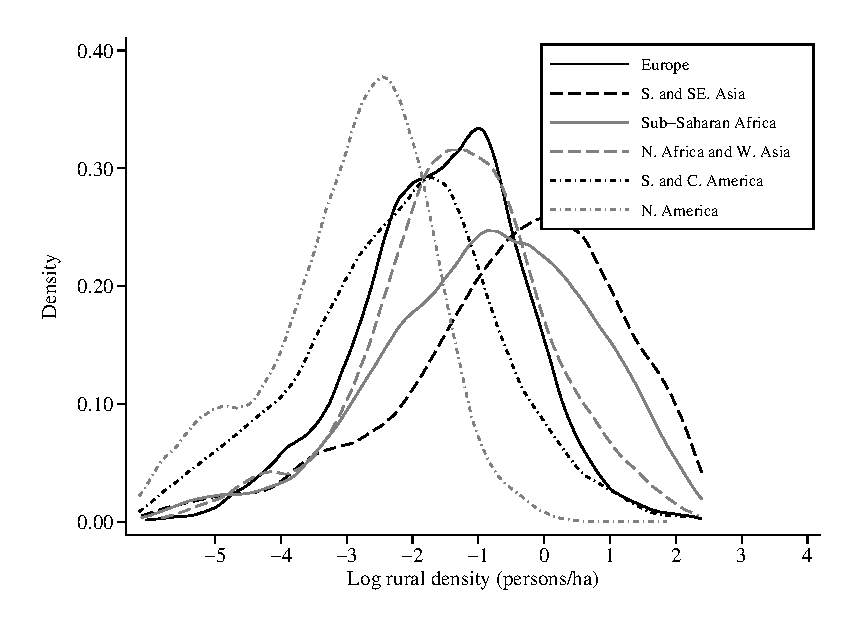
\includegraphics[width=1.0\textwidth]{fig_dens_rurd.eps}
\end{center}
\vspace{-.5cm}\singlespacing {\footnotesize \textbf{Notes}: Kernel density plot, Epanechnikov kernel, of the (log) rural density, $L_{Aisc}/X_{isc}$, at the district level, calculated by the authors using data from \citet{hyde31} for rural population. ``Temperate'' includes districts that are suitable for growing barley, buckwheat, oats, rye, wheat, and white potatoes, but have zero suitability for cassava, cowpeas, pearl millet, sweet potato, wet rice, and yams. ``Tropical'' includes districts suitable for the latter set of crops, but zero suitability for the former. 
}
\end{figure}

\clearpage

\begin{figure}[!htb]
\begin{center}
\caption{Density Plot of Caloric Yield ($A^{GAEZ}_{isc}$), by Crop Type}
\label{FIG_dens_csi}
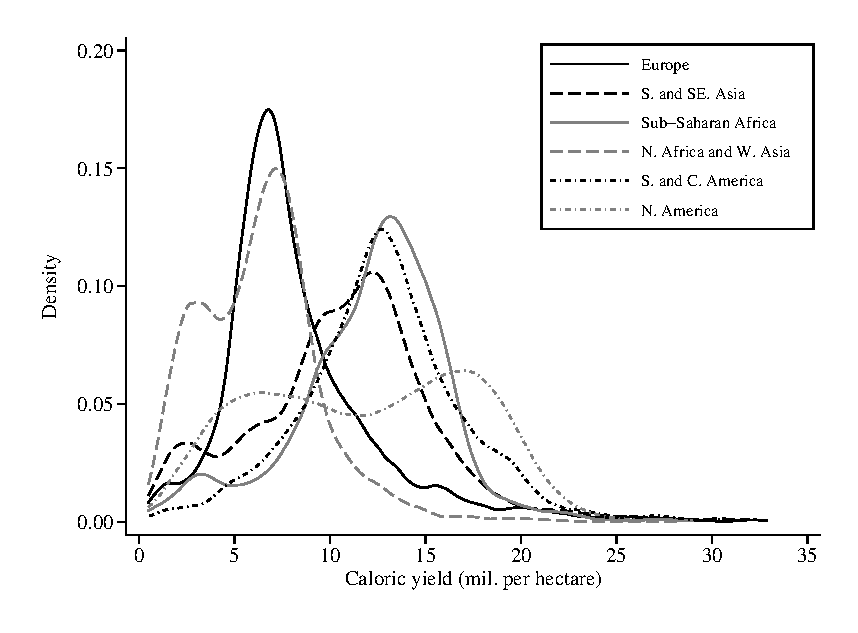
\includegraphics[width=1.0\textwidth]{fig_dens_csi.eps}
\end{center}
\vspace{-.5cm}\singlespacing {\footnotesize \textbf{Notes}: Kernel density plot, Epanechnikov kernel, of the caloric yield, $A_{isc}$, at the district level, calculated by the authors using data from \citet{galorozak2016}. See text for details. This measure sums the maximum calories available per grid cell within a district, then divides by total area of the district. ``Temperate'' includes districts that are suitable for growing barley, buckwheat, oats, rye, wheat, and white potatoes, but have zero suitability for cassava, cowpeas, pearl millet, sweet potato, wet rice, and yams. ``Tropical'' includes districts suitable for the latter set of crops, but zero suitability for the former. 
}
\end{figure}

\clearpage

\begin{figure}[!htb]
\begin{center}
\caption{Residual Relationship of Caloric Yield ($A^{GAEZ}_{isc}$) and Rural Density}
\label{FIG_beta_crop}
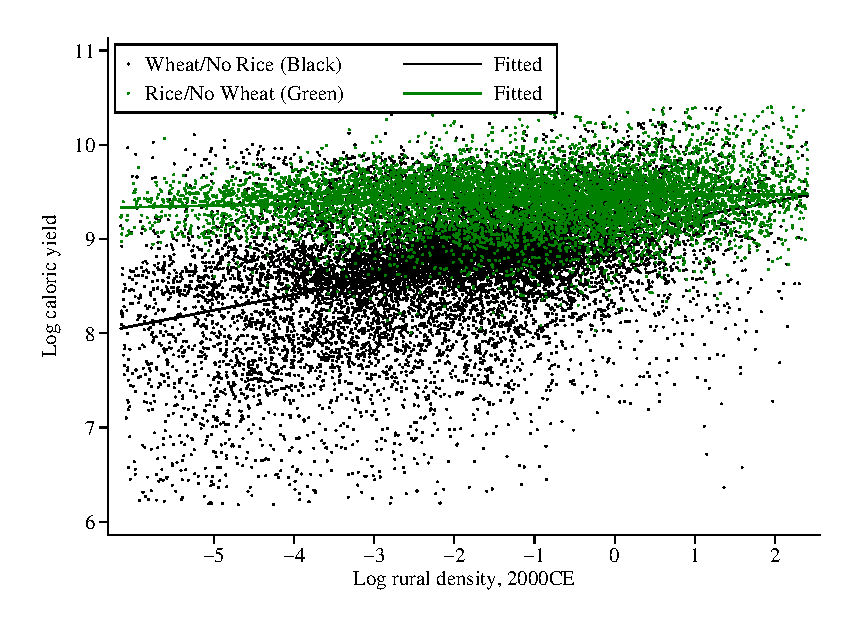
\includegraphics[width=1.0\textwidth]{fig_beta_crop.eps}
\end{center}
\vspace{-.5cm}\singlespacing {\footnotesize \textbf{Notes}: Plotted are the quantile averages of both log caloric yield and log rural density for each sample. 50 quantiles are used in each sample. The quantiles are taken from the residuals of caloric yield and rural density after controlling for log light density, urban percentage in 2000, and province fixed effects. Average values of log caloric yield and log rural density are added back to all residual. Linear fits are shown, and the estimated slopes are in the legend. The \texttt{binscatter} command from Stata was used to prepare the figure. ``Temperate'' includes districts that are suitable for growing barley, buckwheat, oats, rye, wheat, and white potatoes, but have zero suitability for cassava, cowpeas, pearl millet, sweet potato, wet rice, and yams. ``Tropical'' includes districts suitable for the latter set of crops, but with zero suitability for the former. 
}
\end{figure}

\clearpage


\begin{table}[!htb]
\begin{center}
\caption{Summary Statistics for District Level Data, 2000CE}
\label{TAB_summ}
{\small
\begin{tabularx}{\textwidth}{lXXXXXXX}
\midrule
 &      &            & \multicolumn{5}{c}{Percentiles:} \\ \cmidrule{4-8}
 & Mean & SD  & 10th    & 25th    & 50th & 75th & 90th \\
\midrule
Labor/land (persons/ha) &     0.73&     1.17&     0.04&     0.12&     0.32&     0.77&     1.86\\
Caloric yield (mil cals/ha) &    10.85&     4.89&     4.98&     7.17&    10.65&    13.86&    17.03\\
Log light density &    -2.82&     2.93&    -6.14&    -3.83&    -2.51&    -0.89&     0.35\\

\midrule
\end{tabularx}
}
\end{center}
\vspace{-.5cm}\singlespacing {\footnotesize \textbf{Notes}: A total of\districts \ observations for each variable (these come from\provinces \ provinces in\countries \ countries). Caloric yield, $A_{isc}$ calculated by the authors using data from \citet{galorozak2016}. Rural density, $L_{Aisc}/X_{isc}$ calculated by the authors using data from \citet{hyde31} for rural population. Both caloric yield and rural density were trimmed at the 99th and 1st percentiles of their raw data prior to calculating the summary statistics in this table. Urbanization rate taken from \citet{hyde31}. Log mean light density derived from the Global Radiance Calibrated Nightime Lights data provided by NOAA/NGDC, as in \citet{hssw2016}. 
}
\end{table}

\clearpage

\begin{table}[!htb]
\begin{center}
\caption{Estimates of Land Elasticity, $\beta_g$, by Agricultural Type, 2000CE}
\label{TAB_beta_crops}
{\footnotesize
\begin{tabularx}{\textwidth}{lXXXXXX}
\midrule
\multicolumn{7}{l}{Dependent Variable in all panels: Log caloric yield ($A^{GAEZ}_{isg}$)} \\ \\
\multicolumn{7}{l}{Panel A: Regions defined by:} \\ \\
 & \multicolumn{2}{c}{Suitability:} & \multicolumn{2}{c}{Harvest area:} & \multicolumn{2}{c}{Koeppen-Geiger:}\\ \cmidrule(lr){2-3} \cmidrule(lr){4-5} \cmidrule(lr){6-7} 
 & Temperate & Tropical & Temperate  & Tropical  & Temperate  & Tropical \\
 & (1) & (2) & (3) & (4) & (5) & (6) \\
\midrule
Log labor/land ratio ($\beta_g$)&       0.239&       0.088&       0.218&       0.093&       0.220&       0.081\\
                    &     (0.045)&     (0.020)&     (0.039)&     (0.012)&     (0.049)&     (0.016)\\
\midrule
p-value $\beta_g=0$ &       0.000&       0.000&       0.000&       0.000&       0.000&       0.000\\
p-value $\beta_g=\beta_{Temp}$&            &       0.002&            &       0.002&            &       0.007\\
Countries           &          84&          76&          91&         101&          86&          78\\
Observations        &        9404&        7229&       15260&       14794&       10221&       10013\\
R-square (ex. FE)   &        0.24&        0.20&        0.21&        0.18&        0.23&        0.18\\

\midrule
\\
\multicolumn{7}{l}{Panel B: With other restrictions (using suitability to define temperate/tropical)} \\ \\
 & \multicolumn{2}{c}{Urban Pop. $<25K$:} & \multicolumn{2}{c}{Ex. Europe/N. Amer.:} & \multicolumn{2}{c}{Prod $>$ 25th Ptile:}\\ \cmidrule(lr){2-3} \cmidrule(lr){4-5} \cmidrule(lr){6-7}
 & Temperate & Tropical & Temperate  & Tropical  & Temperate  & Tropical \\
 & (1) & (2) & (3) & (4) & (5) & (6) \\
\midrule
Residuals           &       0.257&       0.140&       0.223&       0.131&       0.215&       0.128\\
                    &     (0.022)&     (0.021)&     (0.032)&     (0.018)&     (0.021)&     (0.020)\\
\midrule
p-value $\beta=0$   &       0.000&       0.000&       0.000&       0.000&       0.000&       0.000\\
p-value $\beta=\beta_{Temp}$&            &       0.000&            &       0.009&            &       0.003\\
Countries           &          83&          75&          24&          70&          82&          66\\
Observations        &        7648&        6662&         824&        8826&        8084&        6611\\
Adjusted R-square   &        0.29&        0.24&        0.16&        0.14&        0.24&        0.20\\

\midrule
\end{tabularx}
}
\end{center}
\vspace{-.5cm}\singlespacing {\footnotesize \textbf{Notes}: Conley standard errors, adjusted for spatial auto-correlation with a cutoff distance of 500km, are shown in parentheses. All regressions include province fixed effects, a constant, and controls for the district urbanization rate and log density of district nighttime lights. The coefficient estimate on rural population density indicates the value of $\beta_g$, see equation (\ref{EQ_regress}). Rural population is from HYDE database \citep{hyde31}, and caloric yield is the author's calculations based on the data from \citet{galorozak2016}. Inclusion of districts in the regression is based on the listed criteria related to crop families. See text for details of how temperate and tropical regions are defined in each case.
}
\end{table}

\clearpage

\begin{table}[!htb]
\begin{center}
\caption{Estimates of Land Elasticity, $\beta_g$, Additional Robustness Checks}
\label{TAB_beta_robust}
{\footnotesize
\begin{tabularx}{\textwidth}{lXXXXXX}
\midrule
\multicolumn{7}{l}{Dependent Variable in all panels: Log caloric yield ($A^{GAEZ}_{isg}$)} \\ \\
\multicolumn{7}{l}{Panel A: Different rural population density sources} \\ \\
 & \multicolumn{2}{c}{HYDE 1950:} & \multicolumn{2}{c}{GRUMP:} & \multicolumn{2}{c}{IPUMS:}\\ \cmidrule(lr){2-3} \cmidrule(lr){4-5} \cmidrule(lr){6-7} 
 & Temperate & Tropical & Temperate  & Tropical  & Temperate  & Tropical \\
 & (1) & (2) & (3) & (4) & (5) & (6) \\
\midrule
Log labor/land ratio ($\beta_g$)&       0.227&       0.118&       0.241&       0.088&       0.189&       0.016\\
                    &     (0.015)&     (0.019)&     (0.045)&     (0.020)&     (0.070)&     (0.017)\\
\midrule
p-value $\beta_g=0$ &       0.000&       0.000&       0.000&       0.000&       0.007&       0.348\\
p-value $\beta_g=\beta_{Temp}$&            &       0.000&            &       0.002&            &       0.010\\
Countries           &          84&          75&          84&          76&          23&          24\\
Observations        &        8723&        6754&        9404&        7229&        1104&        2416\\
R-square (ex. FE)   &        0.26&        0.22&        0.24&        0.20&        0.15&        0.11\\

\midrule
\\
\multicolumn{7}{l}{Panel B: Different land assumptions} \\ \\
 & \multicolumn{2}{c}{Cultivated Area:} & \multicolumn{2}{c}{Ex. $>$ 90th Ptile district size:} & \multicolumn{2}{c}{Ex. provinces $<$ 50 dist.:}\\ \cmidrule(lr){2-3} \cmidrule(lr){4-5} \cmidrule(lr){6-7}
 & Temperate & Tropical & Temperate  & Tropical  & Temperate  & Tropical \\
 & (1) & (2) & (3) & (4) & (5) & (6) \\
\midrule
Log rural density ($\beta_g$)   &       0.215&       0.132&       0.215&       0.133&       0.239&       0.105\\
                    &     (0.020)&     (0.020)&     (0.020)&     (0.020)&     (0.028)&     (0.037)\\
\midrule
p-value $\beta_g=0$   &       0.000&       0.000&       0.000&       0.000&       0.000&       0.004\\
p-value $\beta_g=\beta_{Temp}$&            &       0.004&            &       0.004&            &       0.004\\
Countries           &          90&          78&          90&          78&          17&           5\\
Observations        &       10600&        8979&       10600&        8979&        3699&        2500\\
R-square (ex. FE)   &        0.26&        0.22&        0.26&        0.22&        0.33&        0.28\\

\midrule
\end{tabularx}
}
\end{center}
\vspace{-.5cm}\singlespacing {\footnotesize \textbf{Notes}: Temperate and tropical samples are defined by the suitability measures described in Table \ref{TAB_beta_crops}. Conley standard errors, adjusted for spatial auto-correlation with a cutoff distance of 500km, are shown in parentheses. All regressions include province fixed effects, a constant, and controls for the district urbanization rate and log density of district nighttime lights. The coefficient estimate on rural population density indicates the value of $\beta_g$, see equation (\ref{EQ_regress}). Caloric yield is the author's calculations based on the data from \citet{galorozak2016}. In Panel A, the population data used to define rural density differs based on the heading in the table (see text for details). In Panel B, the first set of results use rural population (from HYDE) relative to cultivated land area (as opposed to actual land area) to measure density. The second set drops any district over the 90th percentile in aboslute size, and the third set drops districts from any province that has 50 or fewer districts total.
}
\end{table}

\clearpage

\begin{table}[!htb]
\begin{center}
\caption{Estimates of Land Elasticity, $\beta_g$, Alternative Productivity Measures}
\label{TAB_beta_prod}
{\footnotesize
\begin{tabularx}{\textwidth}{lXXXXXX}
\midrule
\multicolumn{7}{l}{Dependent Variable in all panels: Log caloric yield ($A^{GAEZ}_{isg}$)} \\ \\
\multicolumn{7}{l}{Panel A: Caloric yield based on GAEZ input/water use:} \\ \\
 & \multicolumn{2}{c}{Medium/Irrigated:} & \multicolumn{2}{c}{High/Rain-fed:} & \multicolumn{2}{c}{High/Irrigated:}\\ \cmidrule(lr){2-3} \cmidrule(lr){4-5} \cmidrule(lr){6-7} 
 & Temperate & Tropical & Temperate  & Tropical  & Temperate  & Tropical \\
 & (1) & (2) & (3) & (4) & (5) & (6) \\
\midrule
Log labor/land ratio ($\beta_g$)&       0.254&       0.120&       0.286&       0.132&       0.253&       0.120\\
                    &     (0.050)&     (0.022)&     (0.045)&     (0.025)&     (0.050)&     (0.022)\\
\midrule
p-value $\beta_g=0$ &       0.000&       0.000&       0.000&       0.000&       0.000&       0.000\\
p-value $\beta_g=\beta_{Temp}$&            &       0.014&            &       0.003&            &       0.014\\
Countries           &          72&          67&          72&          67&          72&          67\\
Observations        &        8416&        6731&        8389&        6719&        8416&        6731\\
R-square (ex. FE)   &        0.17&        0.14&        0.18&        0.14&        0.17&        0.14\\

\midrule
\\
\multicolumn{7}{l}{Panel B: Excluding Europe and North America, caloric yield based on GAEZ input/water use:} \\ \\
 & \multicolumn{2}{c}{Medium/Irrigated:} & \multicolumn{2}{c}{High/Rain-fed:} & \multicolumn{2}{c}{High/Irrigated:}\\ \cmidrule(lr){2-3} \cmidrule(lr){4-5} \cmidrule(lr){6-7} 
 & Temperate & Tropical & Temperate  & Tropical  & Temperate  & Tropical \\
 & (1) & (2) & (3) & (4) & (5) & (6) \\
\midrule
Residuals           &       0.236&       0.125&       0.235&       0.136&       0.238&       0.124\\
                    &     (0.037)&     (0.019)&     (0.039)&     (0.019)&     (0.034)&     (0.019)\\
\midrule
p-value $\beta=0$   &       0.000&       0.000&       0.000&       0.000&       0.000&       0.000\\
p-value $\beta=\beta_{Temp}$&            &       0.006&            &       0.017&            &       0.003\\
Countries           &          24&          70&          23&          69&          24&          70\\
Observations        &         824&        8826&         816&        8801&         824&        8826\\
Adjusted R-square   &        0.19&        0.15&        0.17&        0.13&        0.19&        0.15\\

\midrule
\end{tabularx}
}
\end{center}
\vspace{-.5cm}\singlespacing {\footnotesize \textbf{Notes}: Temperate and tropical samples are defined by the suitability measures described in Table \ref{TAB_beta_crops}. Conley standard errors, adjusted for spatial auto-correlation with a cutoff distance of 500km, are shown in parentheses. All regressions include province fixed effects, a constant, and controls for the district urbanization rate and log density of district nighttime lights. The coefficient estimate on rural population density indicates the value of $\beta_g$, see equation (\ref{EQ_regress}). In Panel A, the construction of the $A^{GAEZ}_{isg}$ caloric suitability yield differs across the columns. In (1) and (2), the yield is derived from the underlying GAEZ medium input, irrigated data, and the following columns use the high input, rain-fed data, or the high input, irrigated data, as noted. Panel B is identical, but excludes North American and European countries.
}
\end{table}


\clearpage
\begin{table}[!htb]
\begin{center}
\caption{Panel Estimates of Effect of Population Change, by Land Elasticity}
\label{TAB_pop_panel}
{\footnotesize
\begin{tabularx}{\textwidth}{lXXXXXX}
\midrule
 & \multicolumn{6}{c}{Dependent Variable:} \\ \cmidrule(lr){2-7}
 & \multicolumn{2}{c}{Log GDP per capita} & \multicolumn{2}{c}{Log GDP per worker} & \multicolumn{2}{c}{Log population} \\ \cmidrule(lr){2-3} \cmidrule(lr){4-5} \cmidrule(lr){6-7}
 & $\beta<$Median & $\beta>$Median & $\beta<$Median & $\beta>$Median & $\beta<$Median & $\beta>$Median \\
 & (1) & (2) & (3) & (4) & (5) & (6) \\
\midrule
 & \multicolumn{6}{c}{Panel A:} \\ \cmidrule(lr){2-7}
Mortality rate      &       0.333&       0.723&       0.284&       0.776&      -0.361&      -0.597\\
                    &     (0.271)&     (0.136)&     (0.262)&     (0.145)&     (0.186)&     (0.152)\\
\midrule
p-value $\theta=0$  &       0.220&       0.000&       0.281&       0.000&       0.054&       0.000\\
p-value $\theta=\theta^{Loose}$&           .&       0.199&           .&       0.102&           .&       0.327\\
Countries           &          16&          16&          16&          16&          16&          16\\
Observations        &         128&         128&         128&         128&         128&         128\\

\midrule
\\
 & \multicolumn{6}{c}{Panel B:} \\ \cmidrule(lr){2-7}
Log life expectancy &       0.309&      -2.007&       0.214&      -1.928&       1.910&       1.564\\
                    &     (0.393)&     (0.308)&     (0.387)&     (0.309)&     (0.235)&     (0.229)\\
\midrule
p-value $\theta=0$  &       0.434&       0.000&       0.582&       0.000&       0.000&       0.000\\
p-value $\theta=\theta^{Below}$&           .&       0.000&           .&       0.000&           .&       0.292\\
Countries           &          13&          14&          13&          14&          13&          14\\
Observations        &          99&         106&          99&         106&          99&         106\\

\midrule
\\
 & \multicolumn{6}{c}{Panel C:} \\ \cmidrule(lr){2-7}
Log population      &      -0.380&      -0.776&      -0.383&      -0.763\\
                    &     (0.125)&     (0.067)&     (0.121)&     (0.062)\\
\midrule
p-value $\theta=0$  &       0.003&       0.000&       0.002&       0.000\\
p-value $\theta=\theta^{Below}$&           .&       0.006&           .&       0.006\\
Countries           &          16&          16&          16&          16\\
Observations        &         128&         128&         128&         128\\

\midrule
\end{tabularx}
}
\end{center}
\vspace{-.5cm}\singlespacing {\footnotesize \textbf{Notes}: Robust standard errors are reported in parentheses. All regressions include both year fixed effects and country fixed effects. The value of $\beta$ for each country was found by estimating equation (\ref{EQ_regress}) separately for each, including province-level fixed effects. Countries are then included in a regression here based on how their $\beta$ compares to the median from the 32 countries. The mortality rate used as an explanatory variable in Panel A is the mortality rate from 15 infectious diseases, as documented by \cite{aj07}. All data on GDP per capita, GDP per worker, population, and life expectancy is also taken from those author's dataset. The p-value of $\theta = \theta^{Below}$ is from a test that the estimated coefficient in a column for countries with elasticities above the median is equal to the estimated coefficient of countries below the median.
}
\end{table}



\end{document}